\documentclass[12pt]{report}
%\usepackage{graphicx}
\usepackage[a4paper,top=1in,bottom=1in,left=1.5in,right=1in]{geometry}%margin
\usepackage{graphicx}% for fig
\usepackage{sidecap}%fore side caption of fig
\usepackage{fancyhdr}%for header and footer
\pagestyle{fancy}
\fancyhf{}
\usepackage{wrapfig}
\rhead{Online Training in \LaTex}%header
\lhead{KhCE}

\begin{document}
\tableofcontents
\listoffigures
\listoftables
\chapter{Introduction}
\pagenumbering{roman}
\section{Motivation}
\textbf{Hello World} .My name is Anish.Hello World .My name is AnishHello World .My name is AnishHello World .My name is AnishHello World .My name is AnishHello World .My name is AnishHello World .My name is AnishHello World .My name is AnishHello World .My name is AnishHello World .My name is AnishHello World .My name is AnishHello World .\textit{My name is Anish}Hello World .\textsc{My name is Anish.}

\textbf{\textit{Hello World .My name is AnishHello World .My name is AnishHello World .My name is AnishHello World .My name is AnishHello World .My name is AnishHello World .My name is AnishHello World .My name is AnishHello World .My name is AnishHello World .My name is AnishHello World .My name is AnishHello World .My name is Anish}}

\underline{Hello World .My name is AnishHello World }
\textsc{\textit{Hello}}% yo kina chalena?

$$\overline{Hello world}$$% for overline

%To insert figure
\chapter{Placing Figures and Tables}
\section{Placing Figures in\LaTeX}
Patan Durbar Square is very great place.
Patan Durbar Square is very great place.Patan Durbar Square is very great place.Patan Durbar Square is very great place.Patan Durbar Square is very great place.
\begin{figure}[h]
\centering
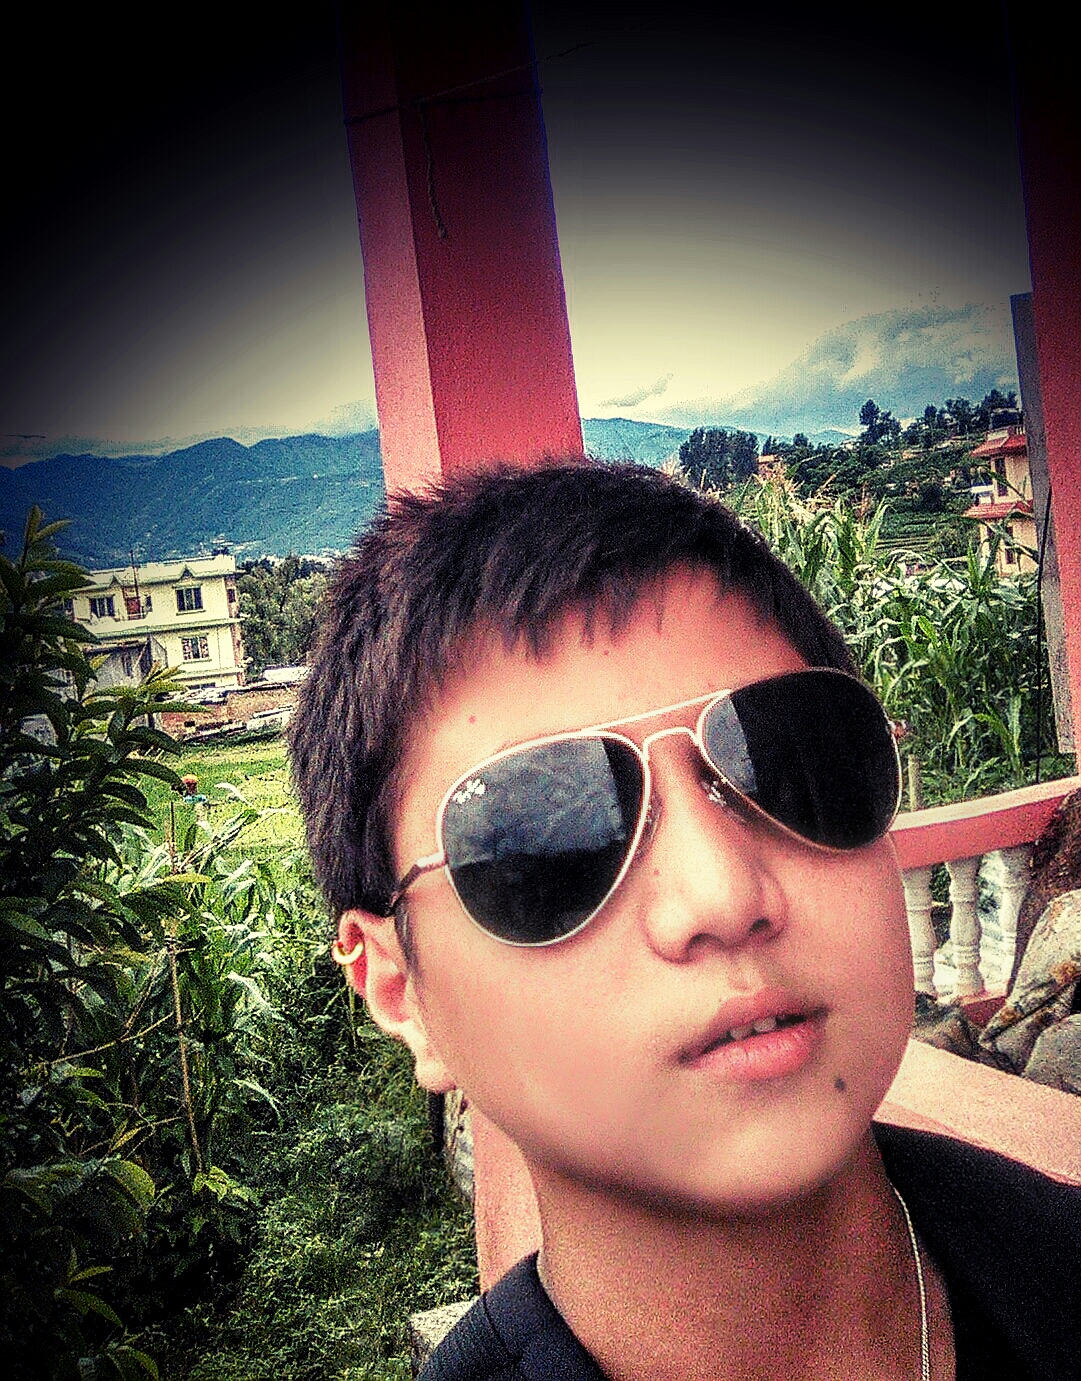
\includegraphics[scale=0.1,angle = 10]{Anish.jpg}
\caption{Patan Durbar Square}
\label{fig:figure1}
\end{figure}

From figure\ref{fig:figure1}
%\begin{figure}[h]
%\centering
%\includegraphics[width=1in,height=1in]%{PatanDurbarSquare.jpg}
%\caption{Patan Durbar Square}
%\end{figure}
\section{abcs}
\chapter{wrappic}

\begin{wrapfigure}{r}{0.25\textwidth}
\centering
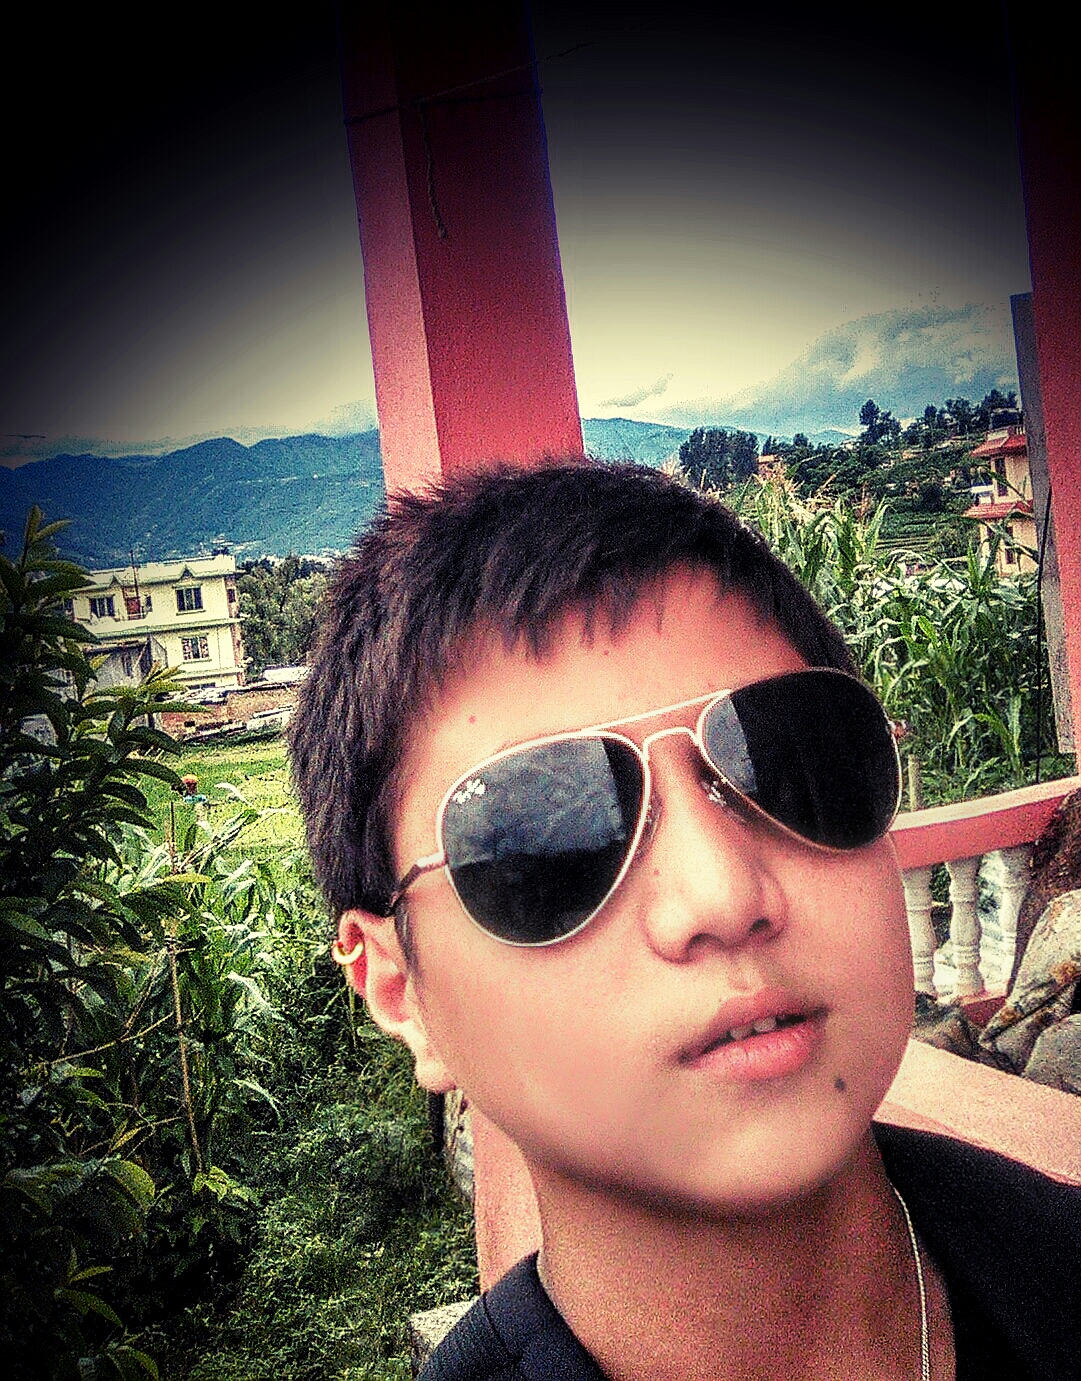
\includegraphics[width = 0.25\textwidth]{Anish.jpg}
\caption{Anish}
\end{wrapfigure}
Mynane is anish.Mynane is anish.Mynane is anish.Mynane is anish.Mynane is anish.Mynane is anish.Mynane is anish.Mynane is anish.Mynane is anish.Mynane is anish.Mynane is anish.Mynane is anish.Mynane is anish.Mynane is anish.Mynane is anish.Mynane is anish.Mynane is anish.Mynane is anish.
%\begin{wrapfigure}{l}{0.25\textwidth}
%\centering
%\includegraphics[width = 0.25\textwidth]%{Anish.jpg}
%\caption{Anish}
%\end{wrapfigure}
Mynane is anish.Mynane is anish.Mynane is anish.Mynane is anish.Mynane is anish.Mynane is anish.Mynane is anish.Mynane is anish.Mynane is anish.Mynane is anish.Mynane is anish.Mynane is anish.Mynane is anish.Mynane is anish.Mynane is anish.Mynane is anish.Mynane is anish.Mynane is anish.
\begin{figure*}[!hbt]
\centering
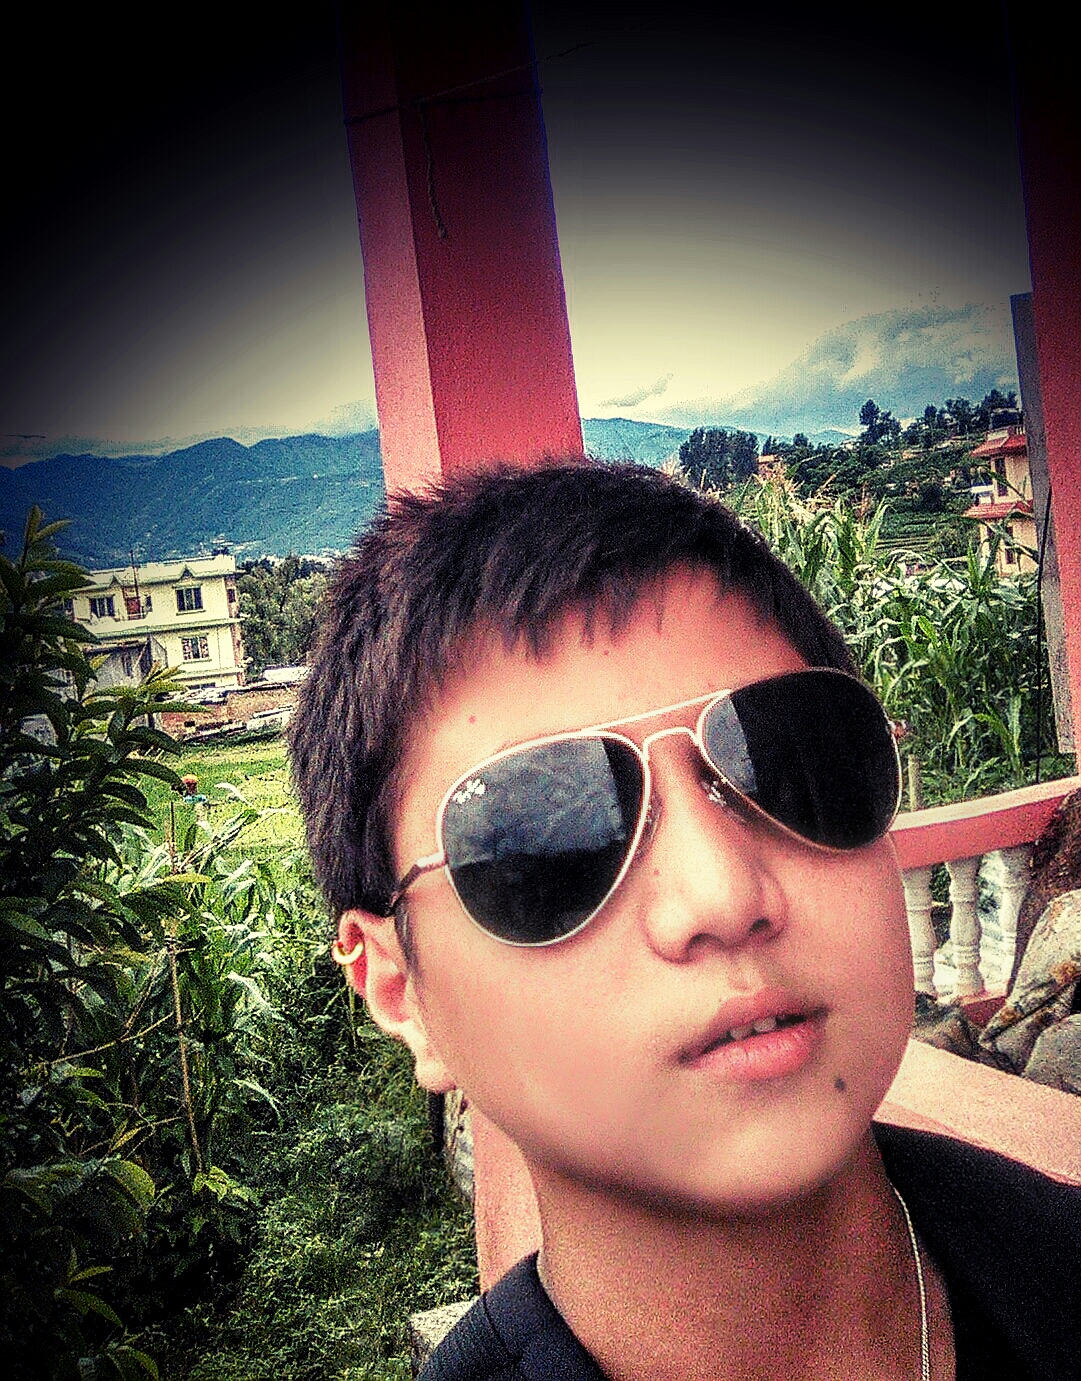
\includegraphics[width=0.1\textwidth]{Anish.jpg}
\caption{Anish Shipakar}
\end{figure*}

%\begin{figure*}{!hbt}
%\centering
%\reflectbox{  % for reflecting
%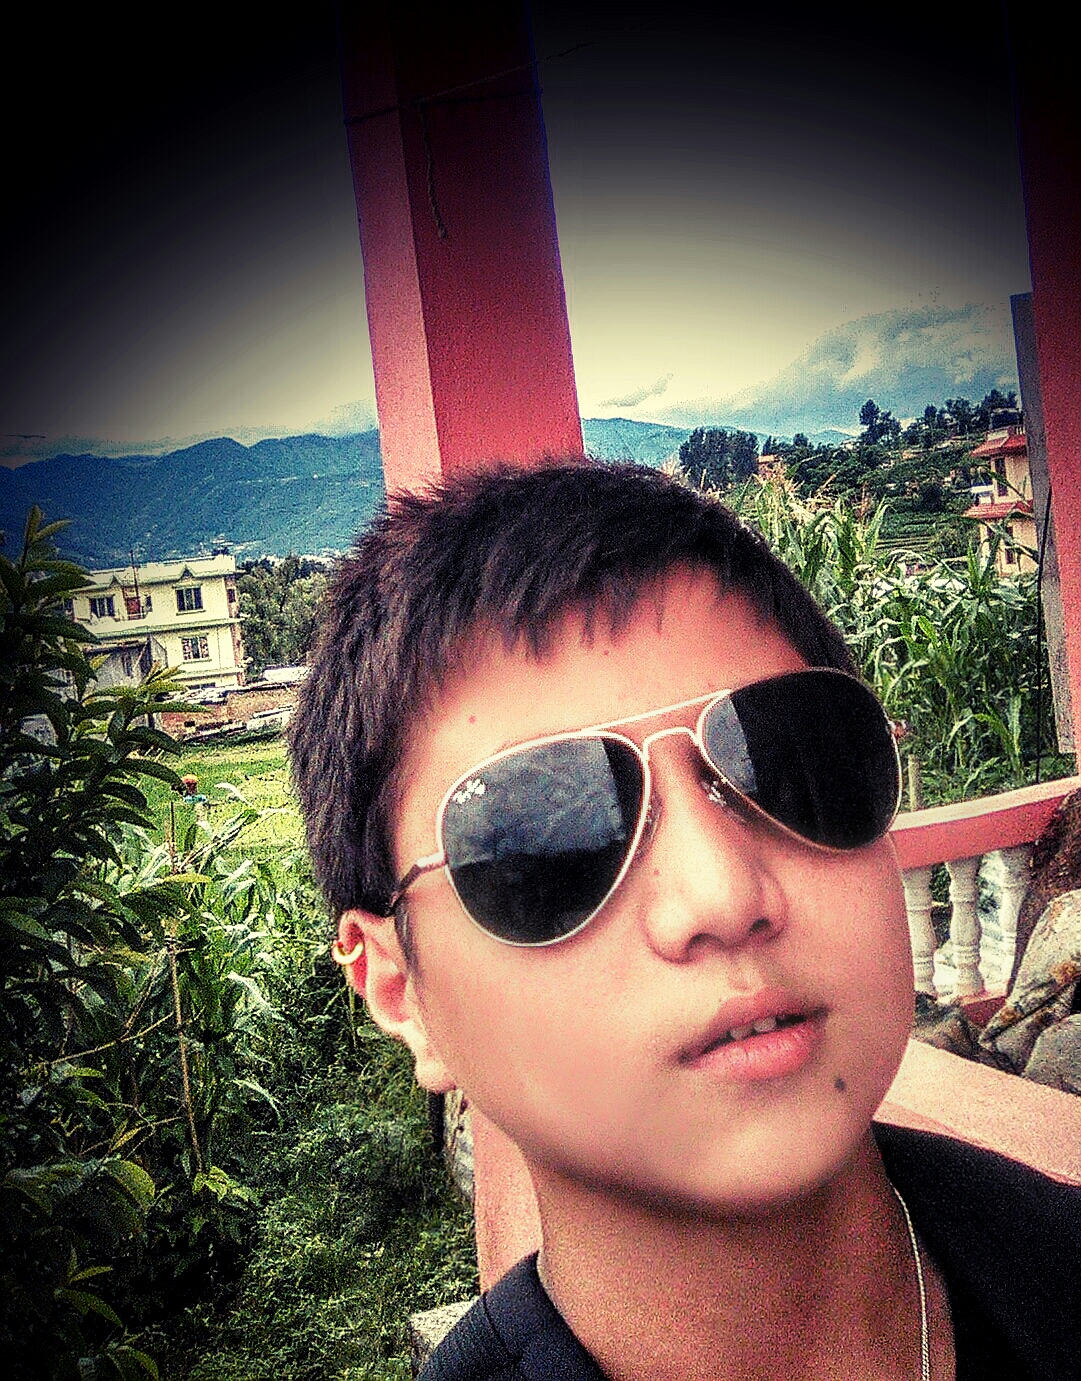
\includegraphics[width=0.5\textwidth]{Anish.jpg}}
%\caption{Anish Shipakar}
%\end{figure*}

\chapter{table}
\section{Placing Tables}
%for managing table
\begin{table}[!hbt]
\centering
\caption{Value of X and Y}
% For creating table
\begin{tabular}{|c|c|}
\hline      % for horizontal line
x & y\\
\hline
1 & 2\\
\hline
3 & 4\\
\hline
5 & 6\\
\hline
\end{tabular}
\end{table}

\begin{table}[!hbt] %!hbt float
\centering
\caption{List of students}
\begin{tabular}{||c|c|c|c|c||}
\hline 
A11 & B & c & d & e \\ 
\hline 
f & g & h & i & j \\ 
\hline 
k & l & m & n & o \\ 
\hline 
p & q & r & s & t \\ 
\hline 
u & v & w & x & y \\ 
\hline 
\end{tabular} 
\end{table}
\chapter{Listing}
\section{numbering}
\begin{enumerate}
\item Computer
   \begin{enumerate}
   \item ram
    \begin{enumerate}
    \item 4 gb
       \begin{enumerate}
       \item cheap
       \item expensive
       \end{enumerate}
    \item 8 gb
   \end{enumerate}
   \item rom
   \end{enumerate}
\item science
\item math
\item english
\end{enumerate}

\section{Listing Using bullet}
\begin{itemize}
\item Computer
   \begin{itemize}
   \item ram % may use \item[symbol]
    \begin{itemize}
    \item 4 gb
       \begin{itemize}
       \item cheap
       \item expensive
       \end{itemize}
    \item 8 gb
   \end{itemize}
   \item rom
   \end{itemize}
\item science
\item math
\item english
\end{itemize}


\end{document}
%use\textbf{•} for bold
%use\textit{ } for italic
%use \textsc{•} for uppercase
%use \underline{•}for underline
%can also use 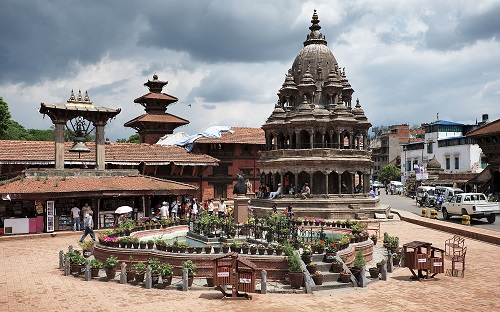
\includegraphics[width=line_width]{patandurbar}no extensiom




